\documentclass[14pt]{extbook}
\usepackage{multicol, enumerate, enumitem, hyperref, color, soul, setspace, parskip, fancyhdr} %General Packages
\usepackage{amssymb, amsthm, amsmath, latexsym, units, mathtools} %Math Packages
\everymath{\displaystyle} %All math in Display Style
% Packages with additional options
\usepackage[headsep=0.5cm,headheight=12pt, left=1 in,right= 1 in,top= 1 in,bottom= 1 in]{geometry}
\usepackage[usenames,dvipsnames]{xcolor}
\usepackage{dashrule}  % Package to use the command below to create lines between items
\newcommand{\litem}[1]{\item#1\hspace*{-1cm}\rule{\textwidth}{0.4pt}}
\pagestyle{fancy}
\lhead{Progress Quiz 10}
\chead{}
\rhead{Version C}
\lfoot{5170-5105}
\cfoot{}
\rfoot{Summer C 2021}
\begin{document}

\begin{enumerate}
\litem{
Solve the quadratic equation below. Then, choose the intervals that the solutions belong to, with $x_1 \leq x_2$ (if they exist).\[ -10x^{2} +9 x + 8 = 0 \]\begin{enumerate}[label=\Alph*.]
\item \( x_1 \in [-20.5, -17.9] \text{ and } x_2 \in [20, 21.7] \)
\item \( x_1 \in [-2.6, -0.9] \text{ and } x_2 \in [-1.4, 1.1] \)
\item \( x_1 \in [-15.1, -13.1] \text{ and } x_2 \in [3.9, 7.3] \)
\item \( x_1 \in [-0.7, 0.3] \text{ and } x_2 \in [0.7, 2.3] \)
\item \( \text{There are no Real solutions.} \)

\end{enumerate} }
\litem{
Solve the quadratic equation below. Then, choose the intervals that the solutions $x_1$ and $x_2$ belong to, with $x_1 \leq x_2$.\[ 15x^{2} -38 x + 24 = 0 \]\begin{enumerate}[label=\Alph*.]
\item \( x_1 \in [1.18, 1.28] \text{ and } x_2 \in [1.19, 1.53] \)
\item \( x_1 \in [18, 18.02] \text{ and } x_2 \in [19.67, 20.4] \)
\item \( x_1 \in [0.32, 0.41] \text{ and } x_2 \in [3.97, 4.38] \)
\item \( x_1 \in [0.57, 0.61] \text{ and } x_2 \in [2.58, 2.84] \)
\item \( x_1 \in [0.65, 0.75] \text{ and } x_2 \in [2.22, 2.5] \)

\end{enumerate} }
\litem{
Graph the equation below.\[ f(x) = -(x+4)^2 + 18 \]\begin{enumerate}[label=\Alph*.]
\begin{multicols}{2}\item 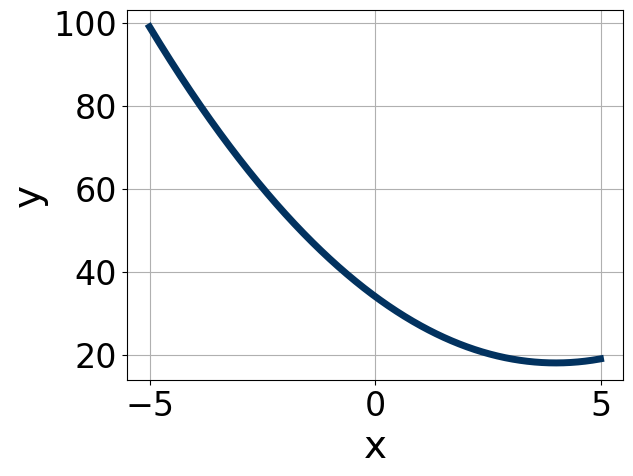
\includegraphics[width = 0.3\textwidth]{../Figures/quadraticEquationToGraphAC.png}\item 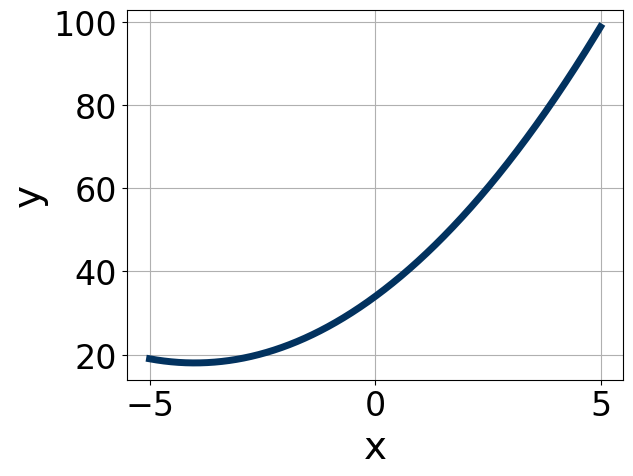
\includegraphics[width = 0.3\textwidth]{../Figures/quadraticEquationToGraphBC.png}\item 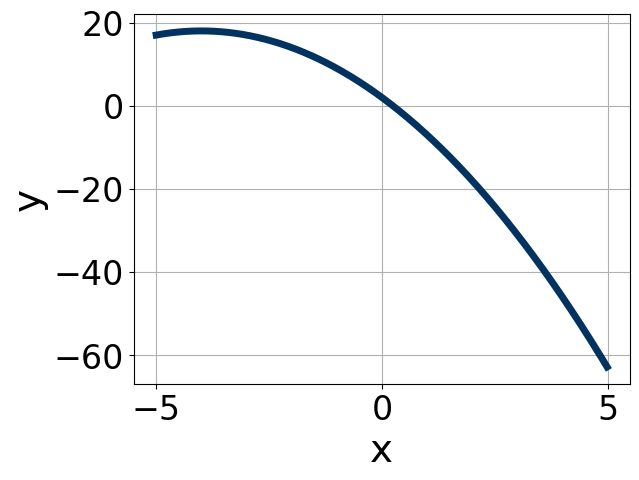
\includegraphics[width = 0.3\textwidth]{../Figures/quadraticEquationToGraphCC.png}\item 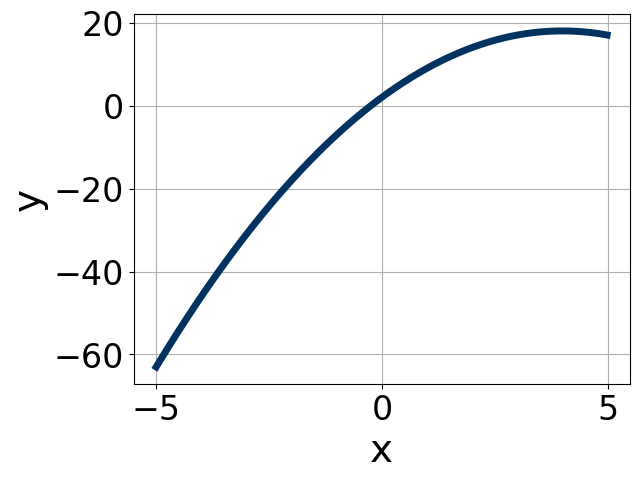
\includegraphics[width = 0.3\textwidth]{../Figures/quadraticEquationToGraphDC.png}\end{multicols}\item None of the above.
\end{enumerate} }
\litem{
Write the equation of the graph presented below in the form $f(x)=ax^2+bx+c$, assuming  $a=1$ or $a=-1$. Then, choose the intervals that $a, b,$ and $c$ belong to.
\begin{center}
    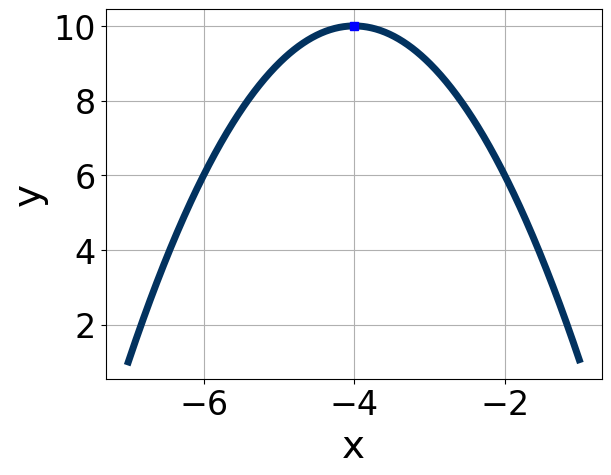
\includegraphics[width=0.5\textwidth]{../Figures/quadraticGraphToEquationC.png}
\end{center}
\begin{enumerate}[label=\Alph*.]
\item \( a \in [-6, 0], \hspace*{5mm} b \in [-9, -7], \text{ and } \hspace*{5mm} c \in [-7, -3] \)
\item \( a \in [-6, 0], \hspace*{5mm} b \in [6, 10], \text{ and } \hspace*{5mm} c \in [-7, -3] \)
\item \( a \in [-6, 0], \hspace*{5mm} b \in [6, 10], \text{ and } \hspace*{5mm} c \in [-27, -24] \)
\item \( a \in [1, 6], \hspace*{5mm} b \in [6, 10], \text{ and } \hspace*{5mm} c \in [24, 28] \)
\item \( a \in [1, 6], \hspace*{5mm} b \in [-9, -7], \text{ and } \hspace*{5mm} c \in [24, 28] \)

\end{enumerate} }
\litem{
Factor the quadratic below. Then, choose the intervals that contain the constants in the form $(ax+b)(cx+d); b \leq d.$\[ 54x^{2} -15 x -25 \]\begin{enumerate}[label=\Alph*.]
\item \( a \in [14.9, 21.4], \hspace*{5mm} b \in [-10, -2], \hspace*{5mm} c \in [1.8, 4.4], \text{ and } \hspace*{5mm} d \in [5, 12] \)
\item \( a \in [1.2, 4.8], \hspace*{5mm} b \in [-10, -2], \hspace*{5mm} c \in [17, 19], \text{ and } \hspace*{5mm} d \in [5, 12] \)
\item \( a \in [0.2, 1.7], \hspace*{5mm} b \in [-46, -43], \hspace*{5mm} c \in [0.4, 2.1], \text{ and } \hspace*{5mm} d \in [28, 31] \)
\item \( a \in [4.5, 8.4], \hspace*{5mm} b \in [-10, -2], \hspace*{5mm} c \in [8.7, 9.5], \text{ and } \hspace*{5mm} d \in [5, 12] \)
\item \( \text{None of the above.} \)

\end{enumerate} }
\litem{
Solve the quadratic equation below. Then, choose the intervals that the solutions $x_1$ and $x_2$ belong to, with $x_1 \leq x_2$.\[ 20x^{2} +61 x + 36 = 0 \]\begin{enumerate}[label=\Alph*.]
\item \( x_1 \in [-5.75, -4.17] \text{ and } x_2 \in [-0.46, -0.4] \)
\item \( x_1 \in [-2.42, -2.3] \text{ and } x_2 \in [-0.77, -0.75] \)
\item \( x_1 \in [-45, -44.45] \text{ and } x_2 \in [-16.02, -15.93] \)
\item \( x_1 \in [-2.26, -1.94] \text{ and } x_2 \in [-0.86, -0.79] \)
\item \( x_1 \in [-9.46, -8.61] \text{ and } x_2 \in [-0.28, -0.13] \)

\end{enumerate} }
\litem{
Write the equation of the graph presented below in the form $f(x)=ax^2+bx+c$, assuming  $a=1$ or $a=-1$. Then, choose the intervals that $a, b,$ and $c$ belong to.
\begin{center}
    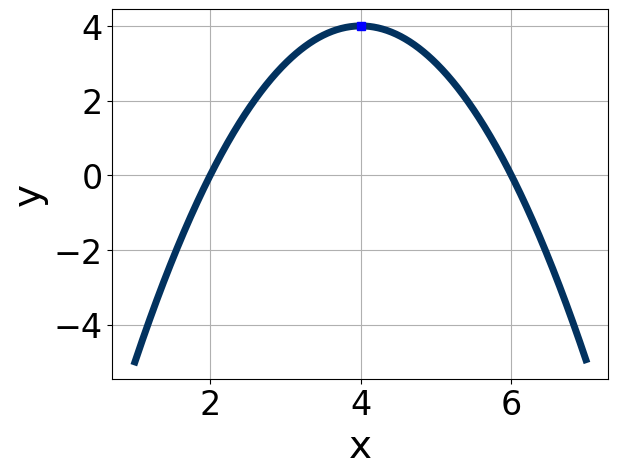
\includegraphics[width=0.5\textwidth]{../Figures/quadraticGraphToEquationCopyC.png}
\end{center}
\begin{enumerate}[label=\Alph*.]
\item \( a \in [-3, 0], \hspace*{5mm} b \in [-10, -7], \text{ and } \hspace*{5mm} c \in [-21, -15] \)
\item \( a \in [0, 3], \hspace*{5mm} b \in [-10, -7], \text{ and } \hspace*{5mm} c \in [19, 21] \)
\item \( a \in [0, 3], \hspace*{5mm} b \in [8, 12], \text{ and } \hspace*{5mm} c \in [19, 21] \)
\item \( a \in [-3, 0], \hspace*{5mm} b \in [8, 12], \text{ and } \hspace*{5mm} c \in [-16, -11] \)
\item \( a \in [-3, 0], \hspace*{5mm} b \in [-10, -7], \text{ and } \hspace*{5mm} c \in [-16, -11] \)

\end{enumerate} }
\litem{
Solve the quadratic equation below. Then, choose the intervals that the solutions belong to, with $x_1 \leq x_2$ (if they exist).\[ 15x^{2} +11 x -9 = 0 \]\begin{enumerate}[label=\Alph*.]
\item \( x_1 \in [-3.2, -0.5] \text{ and } x_2 \in [-0.45, 0.87] \)
\item \( x_1 \in [-27.7, -24.9] \text{ and } x_2 \in [25.18, 25.87] \)
\item \( x_1 \in [-0.9, 1.2] \text{ and } x_2 \in [0.66, 1.65] \)
\item \( x_1 \in [-19.3, -17.4] \text{ and } x_2 \in [7.04, 7.88] \)
\item \( \text{There are no Real solutions.} \)

\end{enumerate} }
\litem{
Factor the quadratic below. Then, choose the intervals that contain the constants in the form $(ax+b)(cx+d); b \leq d.$\[ 16x^{2} +8 x -15 \]\begin{enumerate}[label=\Alph*.]
\item \( a \in [2.63, 4.72], \hspace*{5mm} b \in [-10, 3], \hspace*{5mm} c \in [3.77, 5.84], \text{ and } \hspace*{5mm} d \in [4, 8] \)
\item \( a \in [6.46, 9.19], \hspace*{5mm} b \in [-10, 3], \hspace*{5mm} c \in [1.12, 3.12], \text{ and } \hspace*{5mm} d \in [4, 8] \)
\item \( a \in [0.69, 1.04], \hspace*{5mm} b \in [-18, -11], \hspace*{5mm} c \in [0.84, 1.66], \text{ and } \hspace*{5mm} d \in [15, 22] \)
\item \( a \in [1.68, 2.6], \hspace*{5mm} b \in [-10, 3], \hspace*{5mm} c \in [7.22, 8.16], \text{ and } \hspace*{5mm} d \in [4, 8] \)
\item \( \text{None of the above.} \)

\end{enumerate} }
\litem{
Graph the equation below.\[ f(x) = (x-4)^2 + 16 \]\begin{enumerate}[label=\Alph*.]
\begin{multicols}{2}\item 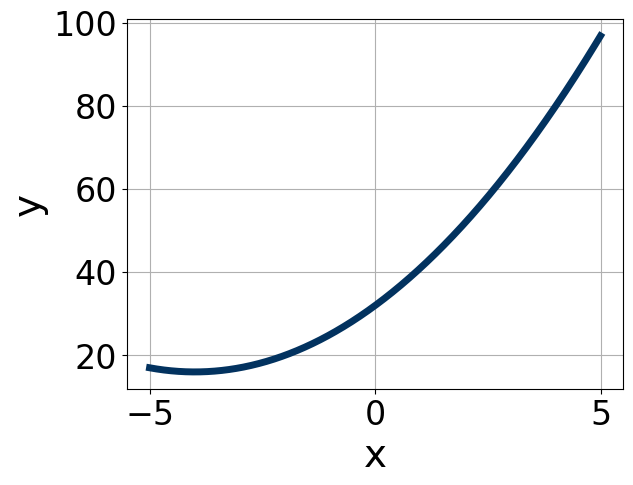
\includegraphics[width = 0.3\textwidth]{../Figures/quadraticEquationToGraphCopyAC.png}\item 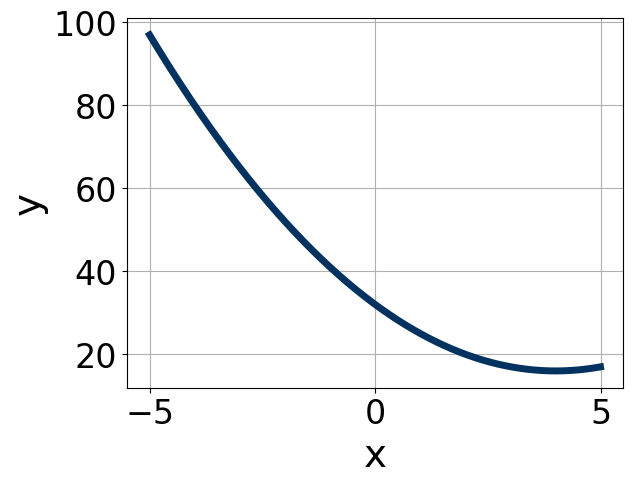
\includegraphics[width = 0.3\textwidth]{../Figures/quadraticEquationToGraphCopyBC.png}\item 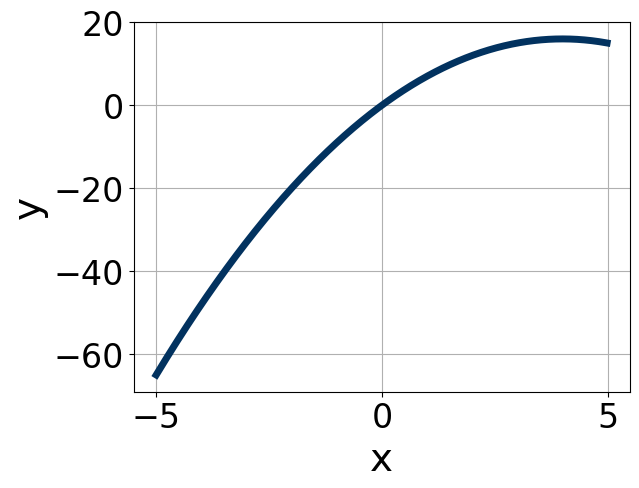
\includegraphics[width = 0.3\textwidth]{../Figures/quadraticEquationToGraphCopyCC.png}\item 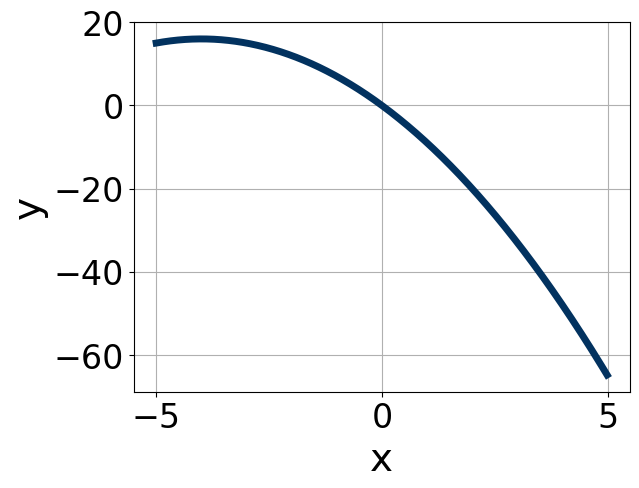
\includegraphics[width = 0.3\textwidth]{../Figures/quadraticEquationToGraphCopyDC.png}\end{multicols}\item None of the above.
\end{enumerate} }
\end{enumerate}

\end{document}